%\VignetteIndexEntry{BICseq HowTo}
%\VignetteKeyword{platform}
%\VignettePackage{BICseq}
\documentclass[12pt]{article}
\usepackage{hyperref}
\usepackage{graphicx}
\textwidth=6.2in
\textheight=8.5in
%\parskip=.3cm
\oddsidemargin=.1in
\evensidemargin=.1in
\headheight=-.3in

\newcommand{\Robject}[1]{{\texttt{#1}}}
\newcommand{\Rfunction}[1]{{\texttt{#1}}}
\newcommand{\Rpackage}[1]{{\textit{#1}}}

\usepackage{Sweave}
\begin{document}
\author{Jianhua Zhang, Ruibin Xi and Peter Park}

\title{How to use BICseq}

\maketitle

\section*{Overview}

The \Rpackage{BICseq} package provides the functionalities for copy number variation (CNV) detection
in whole-genome sequencing data based on the Bayesian Information Criterion (BIC). The algorithm does not assume a parametric model on the read 
distribution on the genome, making it more robust than current available 
methods. It is also fast and able to handle high-coverage genome effectively.

In this vignette, we assume that the BAM files have been sorted and indexed. All
reads in the BAM files will be used for the calculation of CNVs.
If only the uniquely aligned reads are to be used, users are expected to provide 
the BAM files with such data. Work is in progress to add the option of excluding
reads that are not uniquely aligned to the genome. To avoid false positives caused 
by mappability differences among reads of different lengths, we assume all reads in 
the BAM files are of the same length.

\section*{Main functions}

To detect CNVs, a BAM file of a target sample (e. g. tumor 
tissue) and a BAM file of a reference sample (e. g. normal tissue) are needed. 
BICseq assumes that biases in the target sample and the reference sample are the same, and hence the reference sample 
can be used as a control to remove the biases in the target sample.
Warning: Make sure that the target and the reference samples are processed with the same procedure (e.g. with the same number of PCR cycles); 
otherwise, the biases in the target sample and the reference sample may be different and this may result in false positives. 
We are working towards removing the biases in the target sample and the reference sample separately and calling CNVs based on the bias-removed data.

Suppose that the two BAM files are named sample.bam and reference.bam, respectively.
One can create a BICseq object by passing the names of the two BAM files and 
other parameters:

\begin{Schunk}
\begin{Sinput}
> bicseq <- BICseq(sample = sample.bam, reference =reference.bam,  
+     seqNames = c(1:22, "X", "Y"))
\end{Sinput}
\end{Schunk}
where \textit{seqNames} is the vector of the reference sequence names defined in the headers 
of the BAM files.

The \Robject{bicseq} object can then be passed to the \Rfunction{getBICseg} 
function for the detection of genomic alterations:

\begin{Schunk}
\begin{Sinput}
> segs <- getBICseg(object = bicseq, bin = 100, lambda = 2, winSize = 200,  
+     quant = 0.95, mult = 1)
\end{Sinput}
\end{Schunk}
where
\begin{itemize}
\item \textit{bin} = the initial genomic bin size in base pair for read counts; 
    BICseq allows the initial bin size to be 1 bp even for low coverage data, but 
   a smaller bin size would need more memory and computational time. 
\item \textit{lambda} = the penalty of the BIC; 
   a larger lambda will give a smoother profile, i.e. a profile with less breakpoints.
\item the following three parameters are for outlier removal before segmentation. 
\begin{enumerate}
\item \textit{winSize} = the window size for outlier identification; given a genomic 
    position $s$, the genomic window is chosen as $(a,b)$ such that both $(a,s)$ 
    and $(s,b)$ contain at least \textit{winSize}/2 genomic positions that have at 
    least one read aligned.
\item \textit{quant} = the probability of the read count quantile.
\item \textit{mult} = a positive number; a genomic position $s$ is considered as an 
    outlier if it has more than \textit{mult}*\textit{quantile} number of aligned 
    reads, where quantile is the \textit{quant}$^{th}$ quantile of the read counts 
    calculated from the genomic window of $s$. If $s$ is determined as an outlier, 
    BICseq will set the read count at $s$ as \textit{mult}*\textit{quantile}.
\end{enumerate}
\end{itemize}

The \textit{lambda} parameter is the major parameter of BICseq. A larger \textit{lambda} gives CNV calls with fewer false discoveries, 
while a smaller \textit{lambda} is more sensitive. To obtain optimal results, CNVs should be first filtered by a copy ratio threshold.
For low coverage data (< 1X), a smaller \textit{lambda} (e.g. 1 or 1.2) can achieve good sensitivity. 
To further reduce false discovery rate, one can apply a p-value threshold to remove the less significant CNVs.
For medium coverage (2-5X), a larger \textit{lambda} should work well with no additional p-value filtering.
For high coverage (5X-30X), \textit{lambda}=4 should give very confident call while still detecting many small CNVs. If the data is very noisy 
(e.g. two samples have different biases), one can choose very large \textit{lambda} (e.g. 100), 
though this will result in low sensitivity in detecting small CNVs.

The plot function allows for viewing the data points and detected segmentations:

\begin{Schunk}
\begin{Sinput}
> plot(segs, sampleName = "Demo", save = FALSE, 
+     plotBin=TRUE, chromOrder=c(1:22, "X", "Y"))
\end{Sinput}
\end{Schunk}

\begin{figure}[htbp]
  \begin{center}
    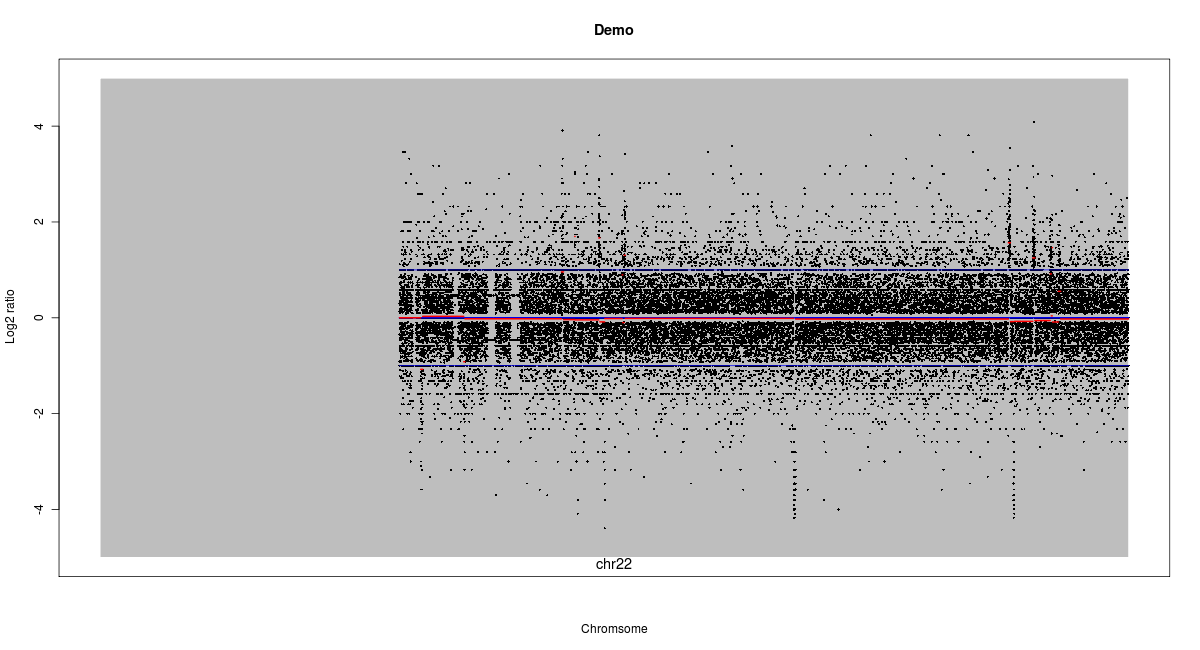
\includegraphics[scale=0.5]{fig01}
    \caption{An example plot showing the genomic alterations.
    Black dots are log2 ratios of sample/reference read counts and red lines are the detected segmentations.}
  \end{center}
\end{figure}

By setting \textit{save} to TRUE, a temporay png file will be generated with the path 
to the file returned by the function. 
The option \textit{plotBin} specifies whether or not the log2 copy ratios in the initial bins should be plotted. 
Since plotting the initial bins is slow for a large genome with a small initial bin size, one may turn off this feature by setting \textit{plotBin} to FALSE.
The plotting order of the chromosomes is determined by the option \textit{chromOrder}. 
This option can contain only a subset of all chromosomes, in which case only the given chromosomes will be plotted.

The \Robject{segs} object contains both read counts in bins and the 
segmentation. The log2 copy ratios of the bins can be obtained by:

\begin{Schunk}
\begin{Sinput}
> bins <- BICseq:::getRatios(bin(segs), what = "bin")
\end{Sinput}
\end{Schunk}

One may get the the segmentation statistics like pvalues, read counts, log2 copy ratios with the following:

\begin{Schunk}
\begin{Sinput}
> seg.summary <- BICseq:::getSummary(segs,correction=TRUE)
\end{Sinput}
\end{Schunk}
By setting \textit{correction} to TRUE, the pvalues will be corrected by Bonferroni's method.

\end{document}








